% ================================================================
% The printable version of latex/starters/retrieval/lessPriorKnowledge/crossTopic/shapeAndAveragesStarters_retrieveAndConnect.tex
%
% This is the same deck, laid out to be handed out rather than put on
% the board. Every slide is shown as it stands before any answer is
% revealed, and 4 copies of it go on one page of A4, two by two, so
% that a printed page cuts into four question sheets.
%
%   made from           latex/starters/retrieval/lessPriorKnowledge/crossTopic/shapeAndAveragesStarters_retrieveAndConnect.tex
%   slides on the sheet 2
%   copies of each      4, two by two on A4 landscape
%   printing rules      version 2
%
% Nothing was reworded and nothing was rewritten. Each slide is the slide
% from the deck, asked for at its first step, which is how the answers
% stay hidden.
%
% Please don't edit this file. It is written again from the one it was
% made from whenever that changes, so an edit here would be lost - edit
% that file instead and this one follows.
% ================================================================
% ================================================================
% The Retrieve and Connect version of latex/starters/retrieval/lessPriorKnowledge/crossTopic/shapeAndAveragesStarters.tex
%
% This is the same deck as the one above, made by renaming the titles in it.
% Every slide that was a numbered starter is now titled
% "Retrieve and Connect", and the word is renamed wherever else a title
% used it. Nothing outside a title has been changed.
%
%   made from           latex/starters/retrieval/lessPriorKnowledge/crossTopic/shapeAndAveragesStarters.tex
%   retitling rules     version 1
%
% Please don't edit this file. It is written again from the one it was
% made from whenever that changes, so an edit here would be lost - edit
% that file instead and this one follows.
% ================================================================
\documentclass{beamer}
\usepackage{tikz}
\usetikzlibrary{calc,arrows.meta}
\usepackage{xcolor}
\usepackage{multicol}
\usepackage{amsmath}

% ================================================================
% Answer-overlay helpers
% ================================================================
\newcommand{\ablank}[1]{%
  \alt<2>{\textcolor{red}{#1}}{\underline{\phantom{#1}}}%
}
\newcommand{\ashow}[1]{\uncover<2->{\textcolor{red}{\small #1}}}
\newcommand{\ashowq}[1]{\alt<2->{\textcolor{red}{\small #1}}{?}}

% Answers drawn straight on to a TikZ diagram, revealed on overlay 2 like \ashow.
% Space is reserved on overlay 1, so the diagram does not move between slides.
\usetikzlibrary{overlay-beamer-styles}
\tikzset{
  ans/.style     = {red, thick, visible on=<2->},
  ansfill/.style = {red!15, visible on=<2->},
  anslab/.style  = {red, font=\tiny, visible on=<2->},
}

\title{Areas, Perimeters \& Averages}
\author{}
\date{}

% ---------------------------------------------------------------
% Added so this deck prints four slides to a page. Nothing above
% this line was changed.
% ---------------------------------------------------------------
\usepackage{pgfpages}

% 4 slides to a sheet of A4, two by two, with a thin line round each
% so that the page can be cut up.
%
% Each slide keeps a margin of 1mm around it and no more, so the four fill
% the sheet and the pieces they cut into are as big as the paper allows. Only
% one direction actually comes out that tight: a slide is a different shape
% from a quarter of a sheet of A4, so it is scaled to fit and the slack it
% cannot use is left along whichever pair of edges it did not fill.
\pgfpagesuselayout{4 on 1}[a4paper,landscape,border shrink=1mm]
\pgfpageslogicalpageoptions{1}{border code=\pgfusepath{stroke}}
\pgfpageslogicalpageoptions{2}{border code=\pgfusepath{stroke}}
\pgfpageslogicalpageoptions{3}{border code=\pgfusepath{stroke}}
\pgfpageslogicalpageoptions{4}{border code=\pgfusepath{stroke}}

% There is nothing on paper to click, and a slide announcing a new section
% would sit between two copies of the same question and put every page after
% it out of step with the grid.
\setbeamertemplate{navigation symbols}{}
\AtBeginPart{}
\AtBeginSection{}
\AtBeginSubsection{}
\AtBeginSubsubsection{}
\begin{document}

\frame{\titlepage}

%------------------------------------------------
% SLIDE 1: Areas, Perimeters, Mean & Fractions
%------------------------------------------------
\begin{frame}<1>{Retrieve and Connect}

\vspace{-1em}

\begin{columns}

\column{0.38\textwidth}
\begin{center}
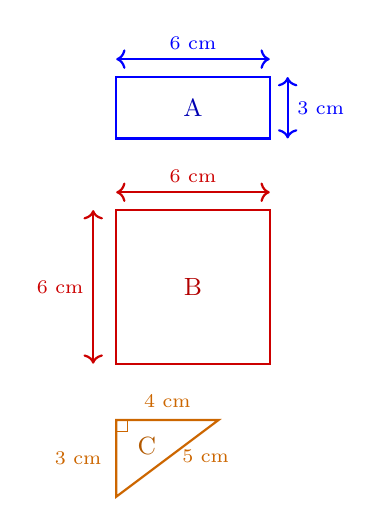
\begin{tikzpicture}[scale=0.65]

  %--- Shape A: Rectangle, 6 cm × 3 cm ---
  \draw[thick, blue] (0,9.5) rectangle (3,8.3);
  \draw[blue, thick, <->] (0,9.85) -- (3,9.85);
  \node[blue, above] at (1.5,9.85) {\scriptsize 6 cm};
  \draw[blue, thick, <->] (3.35,8.3) -- (3.35,9.5);
  \node[blue, right] at (3.35,8.9) {\scriptsize 3 cm};
  \node[blue!70!black] at (1.5,8.9) {\small A};

  %--- Shape B: Square, 6 cm × 6 cm ---
  \draw[thick, red!80!black] (0,6.9) rectangle (3,3.9);
  \draw[red!80!black, thick, <->] (0,7.25) -- (3,7.25);
  \node[red!80!black, above] at (1.5,7.25) {\scriptsize 6 cm};
  \draw[red!80!black, thick, <->] (-0.45,3.9) -- (-0.45,6.9);
  \node[red!80!black, left] at (-0.45,5.4) {\scriptsize 6 cm};
  \node[red!70!black] at (1.5,5.4) {\small B};

  %--- Shape C: Right-angled triangle, legs 4 cm and 3 cm, hypotenuse 5 cm ---
  % Vertices: right angle at (0,2.8), base to (2,2.8), height down to (0,1.3)
  \draw[thick, orange!80!black] (0,2.8) -- (2,2.8) -- (0,1.3) -- cycle;
  % Right angle mark at (0,2.8)
  \draw[orange!80!black] (0.22,2.8) -- (0.22,2.58) -- (0,2.58);
  % Labels
  \node[orange!80!black, above] at (1.0,2.85) {\scriptsize 4 cm};
  \node[orange!80!black, left] at (-0.1,2.05) {\scriptsize 3 cm};
  % Hypotenuse label: midpoint of (2,2.8)--(0,1.3) = (1, 2.05)21
  \node[orange!80!black, right] at (1.1,2.1) {\scriptsize 5 cm};
  \node[orange!70!black] at (0.6,2.3) {\small C};

\end{tikzpicture}
\end{center}

\column{0.62\textwidth}
\small
\begin{enumerate}
  \begin{multicols}{2}
    \item $6 \times 3 =$ \ashowq{$18$}
    \item $\frac{3}{24} + \frac{5}{24} =$ \ashowq{$\frac{1}{3}$}
  \end{multicols}
  \begin{multicols}{2}
    \item $\tfrac{1}{2} \times 4 \times 3 =$ \ashowq{$6$}
    \item $-3 \times -2 =$ \ashowq{$6$}
  \end{multicols}
  \item Find the mean of $\ 8,\ 14,\ 20$. \ashow{$14$}
  \item What fraction of $60$ is $6$?\quad Simplify fully. \ashow{$\frac{1}{10}$}
\end{enumerate}

\vspace{-1.2em}

\begin{enumerate}
  \setcounter{enumi}{6}
  \item Find the \textbf{area} of each shape A, B and C. \ablank{$A=18$},\ \ablank{$B=36$},\ \ablank{$C=6$}.
  \item Find the \textbf{perimeter} of each shape A, B and C. \ablank{$A=18$},\ \ablank{$B=24$},\ \ablank{$C=12$}.
  \item Find the \textbf{mean area} of the three shapes. \ablank{$20$}.
  \item Find the \textbf{mean perimeter} of the three shapes. \ablank{$18$}.
  \item What fraction of the total area does shape C make up? \ablank{$\frac{6}{60}=\frac{1}{10}$}.
\end{enumerate}

\end{columns}
\end{frame}
\begin{frame}<1>{Retrieve and Connect}

\vspace{-1em}

\begin{columns}

\column{0.38\textwidth}
\begin{center}
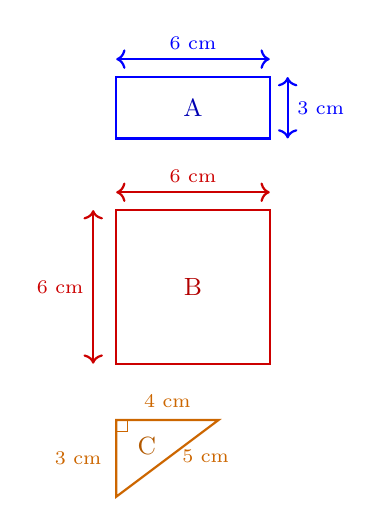
\begin{tikzpicture}[scale=0.65]

  %--- Shape A: Rectangle, 6 cm × 3 cm ---
  \draw[thick, blue] (0,9.5) rectangle (3,8.3);
  \draw[blue, thick, <->] (0,9.85) -- (3,9.85);
  \node[blue, above] at (1.5,9.85) {\scriptsize 6 cm};
  \draw[blue, thick, <->] (3.35,8.3) -- (3.35,9.5);
  \node[blue, right] at (3.35,8.9) {\scriptsize 3 cm};
  \node[blue!70!black] at (1.5,8.9) {\small A};

  %--- Shape B: Square, 6 cm × 6 cm ---
  \draw[thick, red!80!black] (0,6.9) rectangle (3,3.9);
  \draw[red!80!black, thick, <->] (0,7.25) -- (3,7.25);
  \node[red!80!black, above] at (1.5,7.25) {\scriptsize 6 cm};
  \draw[red!80!black, thick, <->] (-0.45,3.9) -- (-0.45,6.9);
  \node[red!80!black, left] at (-0.45,5.4) {\scriptsize 6 cm};
  \node[red!70!black] at (1.5,5.4) {\small B};

  %--- Shape C: Right-angled triangle, legs 4 cm and 3 cm, hypotenuse 5 cm ---
  % Vertices: right angle at (0,2.8), base to (2,2.8), height down to (0,1.3)
  \draw[thick, orange!80!black] (0,2.8) -- (2,2.8) -- (0,1.3) -- cycle;
  % Right angle mark at (0,2.8)
  \draw[orange!80!black] (0.22,2.8) -- (0.22,2.58) -- (0,2.58);
  % Labels
  \node[orange!80!black, above] at (1.0,2.85) {\scriptsize 4 cm};
  \node[orange!80!black, left] at (-0.1,2.05) {\scriptsize 3 cm};
  % Hypotenuse label: midpoint of (2,2.8)--(0,1.3) = (1, 2.05)21
  \node[orange!80!black, right] at (1.1,2.1) {\scriptsize 5 cm};
  \node[orange!70!black] at (0.6,2.3) {\small C};

\end{tikzpicture}
\end{center}

\column{0.62\textwidth}
\small
\begin{enumerate}
  \begin{multicols}{2}
    \item $6 \times 3 =$ \ashowq{$18$}
    \item $\frac{3}{24} + \frac{5}{24} =$ \ashowq{$\frac{1}{3}$}
  \end{multicols}
  \begin{multicols}{2}
    \item $\tfrac{1}{2} \times 4 \times 3 =$ \ashowq{$6$}
    \item $-3 \times -2 =$ \ashowq{$6$}
  \end{multicols}
  \item Find the mean of $\ 8,\ 14,\ 20$. \ashow{$14$}
  \item What fraction of $60$ is $6$?\quad Simplify fully. \ashow{$\frac{1}{10}$}
\end{enumerate}

\vspace{-1.2em}

\begin{enumerate}
  \setcounter{enumi}{6}
  \item Find the \textbf{area} of each shape A, B and C. \ablank{$A=18$},\ \ablank{$B=36$},\ \ablank{$C=6$}.
  \item Find the \textbf{perimeter} of each shape A, B and C. \ablank{$A=18$},\ \ablank{$B=24$},\ \ablank{$C=12$}.
  \item Find the \textbf{mean area} of the three shapes. \ablank{$20$}.
  \item Find the \textbf{mean perimeter} of the three shapes. \ablank{$18$}.
  \item What fraction of the total area does shape C make up? \ablank{$\frac{6}{60}=\frac{1}{10}$}.
\end{enumerate}

\end{columns}
\end{frame}
\begin{frame}<1>{Retrieve and Connect}

\vspace{-1em}

\begin{columns}

\column{0.38\textwidth}
\begin{center}
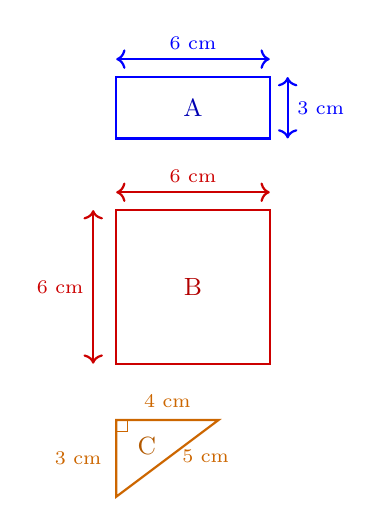
\begin{tikzpicture}[scale=0.65]

  %--- Shape A: Rectangle, 6 cm × 3 cm ---
  \draw[thick, blue] (0,9.5) rectangle (3,8.3);
  \draw[blue, thick, <->] (0,9.85) -- (3,9.85);
  \node[blue, above] at (1.5,9.85) {\scriptsize 6 cm};
  \draw[blue, thick, <->] (3.35,8.3) -- (3.35,9.5);
  \node[blue, right] at (3.35,8.9) {\scriptsize 3 cm};
  \node[blue!70!black] at (1.5,8.9) {\small A};

  %--- Shape B: Square, 6 cm × 6 cm ---
  \draw[thick, red!80!black] (0,6.9) rectangle (3,3.9);
  \draw[red!80!black, thick, <->] (0,7.25) -- (3,7.25);
  \node[red!80!black, above] at (1.5,7.25) {\scriptsize 6 cm};
  \draw[red!80!black, thick, <->] (-0.45,3.9) -- (-0.45,6.9);
  \node[red!80!black, left] at (-0.45,5.4) {\scriptsize 6 cm};
  \node[red!70!black] at (1.5,5.4) {\small B};

  %--- Shape C: Right-angled triangle, legs 4 cm and 3 cm, hypotenuse 5 cm ---
  % Vertices: right angle at (0,2.8), base to (2,2.8), height down to (0,1.3)
  \draw[thick, orange!80!black] (0,2.8) -- (2,2.8) -- (0,1.3) -- cycle;
  % Right angle mark at (0,2.8)
  \draw[orange!80!black] (0.22,2.8) -- (0.22,2.58) -- (0,2.58);
  % Labels
  \node[orange!80!black, above] at (1.0,2.85) {\scriptsize 4 cm};
  \node[orange!80!black, left] at (-0.1,2.05) {\scriptsize 3 cm};
  % Hypotenuse label: midpoint of (2,2.8)--(0,1.3) = (1, 2.05)21
  \node[orange!80!black, right] at (1.1,2.1) {\scriptsize 5 cm};
  \node[orange!70!black] at (0.6,2.3) {\small C};

\end{tikzpicture}
\end{center}

\column{0.62\textwidth}
\small
\begin{enumerate}
  \begin{multicols}{2}
    \item $6 \times 3 =$ \ashowq{$18$}
    \item $\frac{3}{24} + \frac{5}{24} =$ \ashowq{$\frac{1}{3}$}
  \end{multicols}
  \begin{multicols}{2}
    \item $\tfrac{1}{2} \times 4 \times 3 =$ \ashowq{$6$}
    \item $-3 \times -2 =$ \ashowq{$6$}
  \end{multicols}
  \item Find the mean of $\ 8,\ 14,\ 20$. \ashow{$14$}
  \item What fraction of $60$ is $6$?\quad Simplify fully. \ashow{$\frac{1}{10}$}
\end{enumerate}

\vspace{-1.2em}

\begin{enumerate}
  \setcounter{enumi}{6}
  \item Find the \textbf{area} of each shape A, B and C. \ablank{$A=18$},\ \ablank{$B=36$},\ \ablank{$C=6$}.
  \item Find the \textbf{perimeter} of each shape A, B and C. \ablank{$A=18$},\ \ablank{$B=24$},\ \ablank{$C=12$}.
  \item Find the \textbf{mean area} of the three shapes. \ablank{$20$}.
  \item Find the \textbf{mean perimeter} of the three shapes. \ablank{$18$}.
  \item What fraction of the total area does shape C make up? \ablank{$\frac{6}{60}=\frac{1}{10}$}.
\end{enumerate}

\end{columns}
\end{frame}
\begin{frame}<1>{Retrieve and Connect}

\vspace{-1em}

\begin{columns}

\column{0.38\textwidth}
\begin{center}
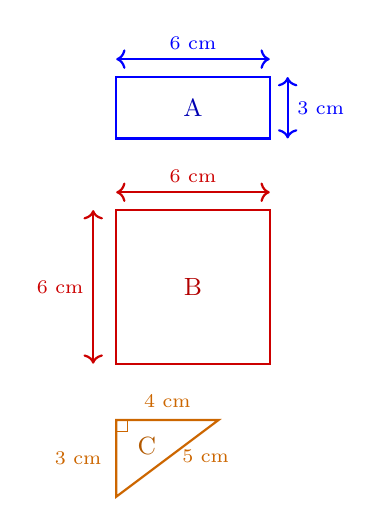
\begin{tikzpicture}[scale=0.65]

  %--- Shape A: Rectangle, 6 cm × 3 cm ---
  \draw[thick, blue] (0,9.5) rectangle (3,8.3);
  \draw[blue, thick, <->] (0,9.85) -- (3,9.85);
  \node[blue, above] at (1.5,9.85) {\scriptsize 6 cm};
  \draw[blue, thick, <->] (3.35,8.3) -- (3.35,9.5);
  \node[blue, right] at (3.35,8.9) {\scriptsize 3 cm};
  \node[blue!70!black] at (1.5,8.9) {\small A};

  %--- Shape B: Square, 6 cm × 6 cm ---
  \draw[thick, red!80!black] (0,6.9) rectangle (3,3.9);
  \draw[red!80!black, thick, <->] (0,7.25) -- (3,7.25);
  \node[red!80!black, above] at (1.5,7.25) {\scriptsize 6 cm};
  \draw[red!80!black, thick, <->] (-0.45,3.9) -- (-0.45,6.9);
  \node[red!80!black, left] at (-0.45,5.4) {\scriptsize 6 cm};
  \node[red!70!black] at (1.5,5.4) {\small B};

  %--- Shape C: Right-angled triangle, legs 4 cm and 3 cm, hypotenuse 5 cm ---
  % Vertices: right angle at (0,2.8), base to (2,2.8), height down to (0,1.3)
  \draw[thick, orange!80!black] (0,2.8) -- (2,2.8) -- (0,1.3) -- cycle;
  % Right angle mark at (0,2.8)
  \draw[orange!80!black] (0.22,2.8) -- (0.22,2.58) -- (0,2.58);
  % Labels
  \node[orange!80!black, above] at (1.0,2.85) {\scriptsize 4 cm};
  \node[orange!80!black, left] at (-0.1,2.05) {\scriptsize 3 cm};
  % Hypotenuse label: midpoint of (2,2.8)--(0,1.3) = (1, 2.05)21
  \node[orange!80!black, right] at (1.1,2.1) {\scriptsize 5 cm};
  \node[orange!70!black] at (0.6,2.3) {\small C};

\end{tikzpicture}
\end{center}

\column{0.62\textwidth}
\small
\begin{enumerate}
  \begin{multicols}{2}
    \item $6 \times 3 =$ \ashowq{$18$}
    \item $\frac{3}{24} + \frac{5}{24} =$ \ashowq{$\frac{1}{3}$}
  \end{multicols}
  \begin{multicols}{2}
    \item $\tfrac{1}{2} \times 4 \times 3 =$ \ashowq{$6$}
    \item $-3 \times -2 =$ \ashowq{$6$}
  \end{multicols}
  \item Find the mean of $\ 8,\ 14,\ 20$. \ashow{$14$}
  \item What fraction of $60$ is $6$?\quad Simplify fully. \ashow{$\frac{1}{10}$}
\end{enumerate}

\vspace{-1.2em}

\begin{enumerate}
  \setcounter{enumi}{6}
  \item Find the \textbf{area} of each shape A, B and C. \ablank{$A=18$},\ \ablank{$B=36$},\ \ablank{$C=6$}.
  \item Find the \textbf{perimeter} of each shape A, B and C. \ablank{$A=18$},\ \ablank{$B=24$},\ \ablank{$C=12$}.
  \item Find the \textbf{mean area} of the three shapes. \ablank{$20$}.
  \item Find the \textbf{mean perimeter} of the three shapes. \ablank{$18$}.
  \item What fraction of the total area does shape C make up? \ablank{$\frac{6}{60}=\frac{1}{10}$}.
\end{enumerate}

\end{columns}
\end{frame}

%------------------------------------------------
% SLIDE 2: Areas, Perimeters, Mean & Fractions
%------------------------------------------------
\begin{frame}<1>{Retrieve and Connect}

\vspace{-1em}

\begin{columns}

\column{0.38\textwidth}
\begin{center}
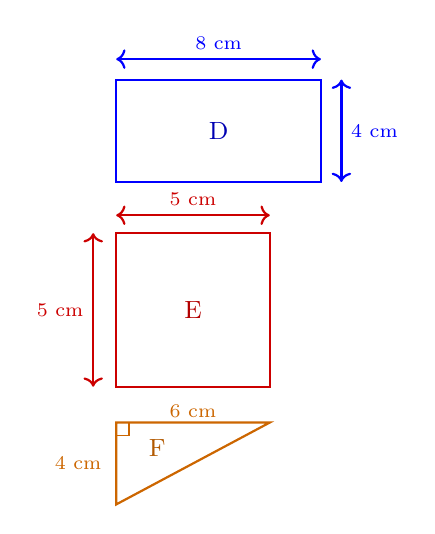
\begin{tikzpicture}[scale=0.65]

  %--- Shape D: Rectangle, 8 cm × 4 cm ---
  \draw[thick, blue] (0,9.5) rectangle (4,7.5);
  \draw[blue, thick, <->] (0,9.9) -- (4,9.9);
  \node[blue, above] at (2,9.9) {\scriptsize 8 cm};
  \draw[blue, thick, <->] (4.4,7.5) -- (4.4,9.5);
  \node[blue, right] at (4.4,8.5) {\scriptsize 4 cm};
  \node[blue!70!black] at (2,8.5) {\small D};

  %--- Shape E: Square, 5 cm × 5 cm ---
  \draw[thick, red!80!black] (0,6.5) rectangle (3,3.5);
  \draw[red!80!black, thick, <->] (0,6.85) -- (3,6.85);
  \node[red!80!black, above] at (1.5,6.85) {\scriptsize 5 cm};
  \draw[red!80!black, thick, <->] (-0.45,3.5) -- (-0.45,6.5);
  \node[red!80!black, left] at (-0.45,5) {\scriptsize 5 cm};
  \node[red!70!black] at (1.5,5) {\small E};

  %--- Shape F: Right-angled triangle, legs 6 cm and 4 cm ---
  \draw[thick, orange!80!black] (0,2.8) -- (3,2.8) -- (0,1.2) -- cycle;
  \draw[orange!80!black] (0.25,2.8) -- (0.25,2.55) -- (0,2.55);
  \node[orange!80!black, above] at (1.5,2.7) {\scriptsize 6 cm};
  \node[orange!80!black, left] at (-0.1,2.0) {\scriptsize 4 cm};
  \node[orange!70!black] at (0.8,2.3) {\small F};

\end{tikzpicture}
\end{center}

\column{0.62\textwidth}
\small
\begin{enumerate}
  \begin{multicols}{2}
    \item $8 \times 4 =$ \ashowq{$32$}
    \item $\frac{7}{20} + \frac{9}{20} =$ \ashowq{$\frac{4}{5}$}
  \end{multicols}
  \begin{multicols}{2}
    \item $\tfrac{1}{2} \times 6 \times 4 =$ \ashowq{$12$}
    \item $-5 \times 4 =$ \ashowq{$-20$}
  \end{multicols}
  \item Find the mean of $\ 6,\ 12,\ 18$. \ashow{$12$}
  \item What fraction of $80$ is $12$?\quad Simplify fully. \ashow{$\frac{3}{20}$}
\end{enumerate}

\vspace{-1.2em}

\begin{enumerate}
  \setcounter{enumi}{6}
  \item Find the \textbf{area} of each shape D, E and F. \ablank{$D=32$},\ \ablank{$E=25$},\ \ablank{$F=12$}.
  \item Find the \textbf{perimeter} of each shape D, E and F. \ablank{$D=24$},\ \ablank{$E=20$},\ \ablank{$F=10+2\sqrt{13}$}.
  \item Find the \textbf{mean area} of the three shapes. \ablank{$23$}.
  \item Find the \textbf{mean perimeter} of the three shapes. \ablank{$\frac{54+2\sqrt{13}}{3}$}.
  \item What fraction of the total area does shape F make up? \ablank{$\frac{12}{69}=\frac{4}{23}$}.
\end{enumerate}

\end{columns}
\end{frame}
\begin{frame}<1>{Retrieve and Connect}

\vspace{-1em}

\begin{columns}

\column{0.38\textwidth}
\begin{center}
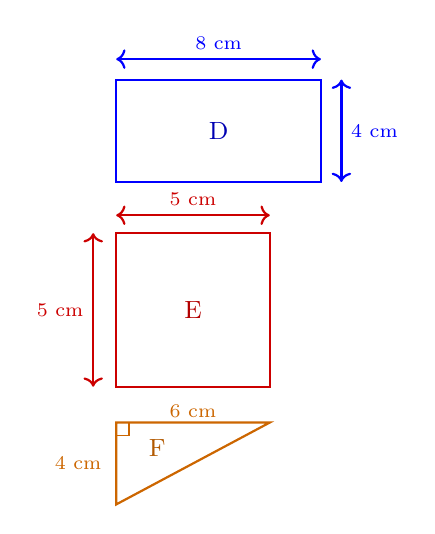
\begin{tikzpicture}[scale=0.65]

  %--- Shape D: Rectangle, 8 cm × 4 cm ---
  \draw[thick, blue] (0,9.5) rectangle (4,7.5);
  \draw[blue, thick, <->] (0,9.9) -- (4,9.9);
  \node[blue, above] at (2,9.9) {\scriptsize 8 cm};
  \draw[blue, thick, <->] (4.4,7.5) -- (4.4,9.5);
  \node[blue, right] at (4.4,8.5) {\scriptsize 4 cm};
  \node[blue!70!black] at (2,8.5) {\small D};

  %--- Shape E: Square, 5 cm × 5 cm ---
  \draw[thick, red!80!black] (0,6.5) rectangle (3,3.5);
  \draw[red!80!black, thick, <->] (0,6.85) -- (3,6.85);
  \node[red!80!black, above] at (1.5,6.85) {\scriptsize 5 cm};
  \draw[red!80!black, thick, <->] (-0.45,3.5) -- (-0.45,6.5);
  \node[red!80!black, left] at (-0.45,5) {\scriptsize 5 cm};
  \node[red!70!black] at (1.5,5) {\small E};

  %--- Shape F: Right-angled triangle, legs 6 cm and 4 cm ---
  \draw[thick, orange!80!black] (0,2.8) -- (3,2.8) -- (0,1.2) -- cycle;
  \draw[orange!80!black] (0.25,2.8) -- (0.25,2.55) -- (0,2.55);
  \node[orange!80!black, above] at (1.5,2.7) {\scriptsize 6 cm};
  \node[orange!80!black, left] at (-0.1,2.0) {\scriptsize 4 cm};
  \node[orange!70!black] at (0.8,2.3) {\small F};

\end{tikzpicture}
\end{center}

\column{0.62\textwidth}
\small
\begin{enumerate}
  \begin{multicols}{2}
    \item $8 \times 4 =$ \ashowq{$32$}
    \item $\frac{7}{20} + \frac{9}{20} =$ \ashowq{$\frac{4}{5}$}
  \end{multicols}
  \begin{multicols}{2}
    \item $\tfrac{1}{2} \times 6 \times 4 =$ \ashowq{$12$}
    \item $-5 \times 4 =$ \ashowq{$-20$}
  \end{multicols}
  \item Find the mean of $\ 6,\ 12,\ 18$. \ashow{$12$}
  \item What fraction of $80$ is $12$?\quad Simplify fully. \ashow{$\frac{3}{20}$}
\end{enumerate}

\vspace{-1.2em}

\begin{enumerate}
  \setcounter{enumi}{6}
  \item Find the \textbf{area} of each shape D, E and F. \ablank{$D=32$},\ \ablank{$E=25$},\ \ablank{$F=12$}.
  \item Find the \textbf{perimeter} of each shape D, E and F. \ablank{$D=24$},\ \ablank{$E=20$},\ \ablank{$F=10+2\sqrt{13}$}.
  \item Find the \textbf{mean area} of the three shapes. \ablank{$23$}.
  \item Find the \textbf{mean perimeter} of the three shapes. \ablank{$\frac{54+2\sqrt{13}}{3}$}.
  \item What fraction of the total area does shape F make up? \ablank{$\frac{12}{69}=\frac{4}{23}$}.
\end{enumerate}

\end{columns}
\end{frame}
\begin{frame}<1>{Retrieve and Connect}

\vspace{-1em}

\begin{columns}

\column{0.38\textwidth}
\begin{center}
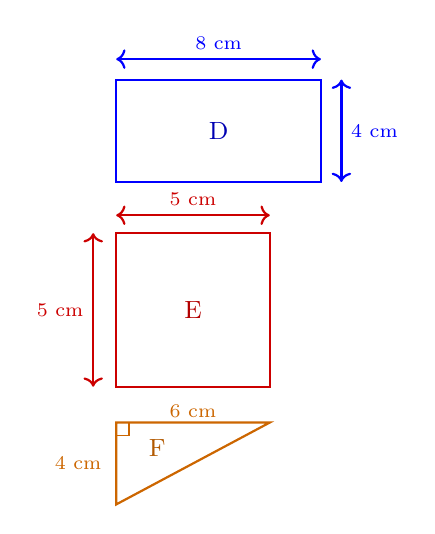
\begin{tikzpicture}[scale=0.65]

  %--- Shape D: Rectangle, 8 cm × 4 cm ---
  \draw[thick, blue] (0,9.5) rectangle (4,7.5);
  \draw[blue, thick, <->] (0,9.9) -- (4,9.9);
  \node[blue, above] at (2,9.9) {\scriptsize 8 cm};
  \draw[blue, thick, <->] (4.4,7.5) -- (4.4,9.5);
  \node[blue, right] at (4.4,8.5) {\scriptsize 4 cm};
  \node[blue!70!black] at (2,8.5) {\small D};

  %--- Shape E: Square, 5 cm × 5 cm ---
  \draw[thick, red!80!black] (0,6.5) rectangle (3,3.5);
  \draw[red!80!black, thick, <->] (0,6.85) -- (3,6.85);
  \node[red!80!black, above] at (1.5,6.85) {\scriptsize 5 cm};
  \draw[red!80!black, thick, <->] (-0.45,3.5) -- (-0.45,6.5);
  \node[red!80!black, left] at (-0.45,5) {\scriptsize 5 cm};
  \node[red!70!black] at (1.5,5) {\small E};

  %--- Shape F: Right-angled triangle, legs 6 cm and 4 cm ---
  \draw[thick, orange!80!black] (0,2.8) -- (3,2.8) -- (0,1.2) -- cycle;
  \draw[orange!80!black] (0.25,2.8) -- (0.25,2.55) -- (0,2.55);
  \node[orange!80!black, above] at (1.5,2.7) {\scriptsize 6 cm};
  \node[orange!80!black, left] at (-0.1,2.0) {\scriptsize 4 cm};
  \node[orange!70!black] at (0.8,2.3) {\small F};

\end{tikzpicture}
\end{center}

\column{0.62\textwidth}
\small
\begin{enumerate}
  \begin{multicols}{2}
    \item $8 \times 4 =$ \ashowq{$32$}
    \item $\frac{7}{20} + \frac{9}{20} =$ \ashowq{$\frac{4}{5}$}
  \end{multicols}
  \begin{multicols}{2}
    \item $\tfrac{1}{2} \times 6 \times 4 =$ \ashowq{$12$}
    \item $-5 \times 4 =$ \ashowq{$-20$}
  \end{multicols}
  \item Find the mean of $\ 6,\ 12,\ 18$. \ashow{$12$}
  \item What fraction of $80$ is $12$?\quad Simplify fully. \ashow{$\frac{3}{20}$}
\end{enumerate}

\vspace{-1.2em}

\begin{enumerate}
  \setcounter{enumi}{6}
  \item Find the \textbf{area} of each shape D, E and F. \ablank{$D=32$},\ \ablank{$E=25$},\ \ablank{$F=12$}.
  \item Find the \textbf{perimeter} of each shape D, E and F. \ablank{$D=24$},\ \ablank{$E=20$},\ \ablank{$F=10+2\sqrt{13}$}.
  \item Find the \textbf{mean area} of the three shapes. \ablank{$23$}.
  \item Find the \textbf{mean perimeter} of the three shapes. \ablank{$\frac{54+2\sqrt{13}}{3}$}.
  \item What fraction of the total area does shape F make up? \ablank{$\frac{12}{69}=\frac{4}{23}$}.
\end{enumerate}

\end{columns}
\end{frame}
\begin{frame}<1>{Retrieve and Connect}

\vspace{-1em}

\begin{columns}

\column{0.38\textwidth}
\begin{center}
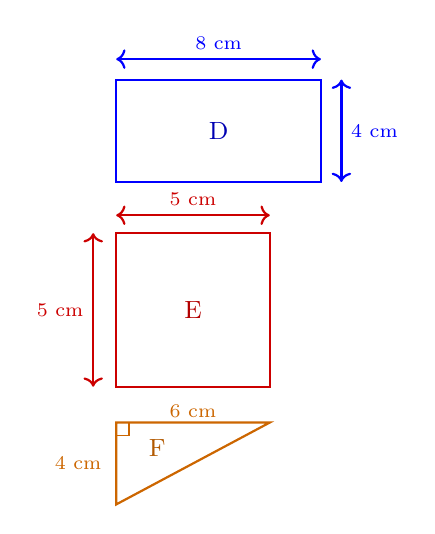
\begin{tikzpicture}[scale=0.65]

  %--- Shape D: Rectangle, 8 cm × 4 cm ---
  \draw[thick, blue] (0,9.5) rectangle (4,7.5);
  \draw[blue, thick, <->] (0,9.9) -- (4,9.9);
  \node[blue, above] at (2,9.9) {\scriptsize 8 cm};
  \draw[blue, thick, <->] (4.4,7.5) -- (4.4,9.5);
  \node[blue, right] at (4.4,8.5) {\scriptsize 4 cm};
  \node[blue!70!black] at (2,8.5) {\small D};

  %--- Shape E: Square, 5 cm × 5 cm ---
  \draw[thick, red!80!black] (0,6.5) rectangle (3,3.5);
  \draw[red!80!black, thick, <->] (0,6.85) -- (3,6.85);
  \node[red!80!black, above] at (1.5,6.85) {\scriptsize 5 cm};
  \draw[red!80!black, thick, <->] (-0.45,3.5) -- (-0.45,6.5);
  \node[red!80!black, left] at (-0.45,5) {\scriptsize 5 cm};
  \node[red!70!black] at (1.5,5) {\small E};

  %--- Shape F: Right-angled triangle, legs 6 cm and 4 cm ---
  \draw[thick, orange!80!black] (0,2.8) -- (3,2.8) -- (0,1.2) -- cycle;
  \draw[orange!80!black] (0.25,2.8) -- (0.25,2.55) -- (0,2.55);
  \node[orange!80!black, above] at (1.5,2.7) {\scriptsize 6 cm};
  \node[orange!80!black, left] at (-0.1,2.0) {\scriptsize 4 cm};
  \node[orange!70!black] at (0.8,2.3) {\small F};

\end{tikzpicture}
\end{center}

\column{0.62\textwidth}
\small
\begin{enumerate}
  \begin{multicols}{2}
    \item $8 \times 4 =$ \ashowq{$32$}
    \item $\frac{7}{20} + \frac{9}{20} =$ \ashowq{$\frac{4}{5}$}
  \end{multicols}
  \begin{multicols}{2}
    \item $\tfrac{1}{2} \times 6 \times 4 =$ \ashowq{$12$}
    \item $-5 \times 4 =$ \ashowq{$-20$}
  \end{multicols}
  \item Find the mean of $\ 6,\ 12,\ 18$. \ashow{$12$}
  \item What fraction of $80$ is $12$?\quad Simplify fully. \ashow{$\frac{3}{20}$}
\end{enumerate}

\vspace{-1.2em}

\begin{enumerate}
  \setcounter{enumi}{6}
  \item Find the \textbf{area} of each shape D, E and F. \ablank{$D=32$},\ \ablank{$E=25$},\ \ablank{$F=12$}.
  \item Find the \textbf{perimeter} of each shape D, E and F. \ablank{$D=24$},\ \ablank{$E=20$},\ \ablank{$F=10+2\sqrt{13}$}.
  \item Find the \textbf{mean area} of the three shapes. \ablank{$23$}.
  \item Find the \textbf{mean perimeter} of the three shapes. \ablank{$\frac{54+2\sqrt{13}}{3}$}.
  \item What fraction of the total area does shape F make up? \ablank{$\frac{12}{69}=\frac{4}{23}$}.
\end{enumerate}

\end{columns}
\end{frame}

\end{document}